%!TEX root = ../master.tex
\chapter{Implementation}\label{ch:implementation}

\section{Tools used}\label{sec:toolsused}
The tools used in this project is an Arduino and the software Pure Data. An Arduino is a micro controller that allows the user to code and create their own circuits using various components. The Arudino is responsible for the control of the physical interface which the user has available.

Pure Data is a visual data flow programming language \cite{puredata} written in C, which is designed for processing audio signals. Pure Data programs, called patches, are written using blocks that represent variable definitions, methods, or other patches. These blocks have inlets and outlets that are then connected to each other to determine the flow of data through the program. Two third party libraries are used with Pure Data; Pduino, which is used to interface with the Arduino, and Gem which adds image processing capabilities to Pure Data. The Firmata firmware is loaded unto the Arduino to enable the Pduino library to communicate with the Arduino.

\subsection{Audio filters}\label{sub:audiofilters}
In the domain of audio effects, the term "filters" describes effects that modify the partial amplitudes of audio signals according to their frequencies \cite{zolzer2011dafx}. Filters combine their input signal with delayed and modified versions of themselves and then filters out certain frequencies. If a delayed version of the input signal is added to the signal, it is called a feedfoward filter, and if the signal is added to a delayed version of itself, it is called a feedback filter. This makes feedback filters more tricky to work with, since their effects can essentially amplify themselves \cite{steiglitz1997digital}. In this case the amplification can continue forever, no matter if you feed the filter a new input signal or not. This continuous amplification is called an unstable filter. Inversely, a stable filter is one, where the response fades over time, tending towards zero. This way you make sure that the response of the input signal will end, depending on how fast the response signal fades.

\begin{figure}
\centering
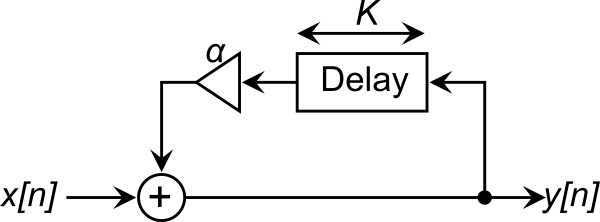
\includegraphics[width=0.5\textwidth]{feedback}
\caption{Structure of basic feedback filter.}
\label{fig:feedback}
\end{figure}

Filters can be put into three basic categories:
\begin{itemize}
\item \textbf{Pass filters} which lets defined frequencies pass, and reject the remaining. Examples of this type of filter are low-pass, bandpass and comb filters.
\item \textbf{Reject Filters} which is the inverse of a Pass filter. With this, defined frequencies are rejected and lets the remaining frequencies pass. Bandreject filters, also known as notch filters, are an example of this.
\item \textbf{Equaliser filters} which changes the amplitude of defined frequencies. This amplitude change can either be positive or negative, depending on the specific implementation of the filter. 
\end{itemize}

The filters used in the project is a bandpass, comb and high-shelf.

The comb filter used is a simple feedback filter, of the structure seen in Figure \ref{fig:feedback}. The summation of the delays creates constructive and destructive interference on the signal. This interference is at regular intervals, which gives the curve of the frequency response its distinct appearance, as seen in Figure \ref{fig:comb}. It is used to give an echo-like effect unto the input signal.

\begin{figure}
\centering
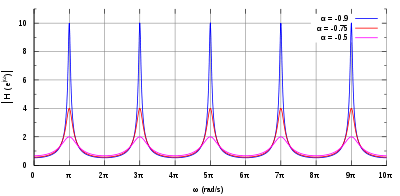
\includegraphics[width=0.5\textwidth]{comb}
\caption{Frequency response curve of a comb filter.}
\label{fig:comb}
\end{figure}

The two other filters used are structured as biquads. This structure consists of two feedforward delays, two feedback delays and a coefficient that is multiplied directly unto the input signal. These five values are then summed to be the output signal. The equation for this operation is 
\[y(n) = b_o \cdot x(n) + b_1 \cdot x(n-1) + b_2 \cdot (n-2) - a_1 \cdot x(n-1) - a_2 \cdot x(n-2)\] \cite{Redmon2003}
where \(x(n)\) is the raw input signal, \(x(n-1)\) is the input signal delayed by one sample, and \(x(n-2)\) is the input signal delayed by two samples. The coefficient \(b_0\) is for the raw input signal, \(b_1\) and \(b_2\) are the coefficients for the feedforward delays, \(a_1\) and \(a_2\) are the coefficients for the feedback delays. This structure, called Direct Form 1, is visualised in Figure \ref{fig:biquadform1}.

\begin{figure}
\centering
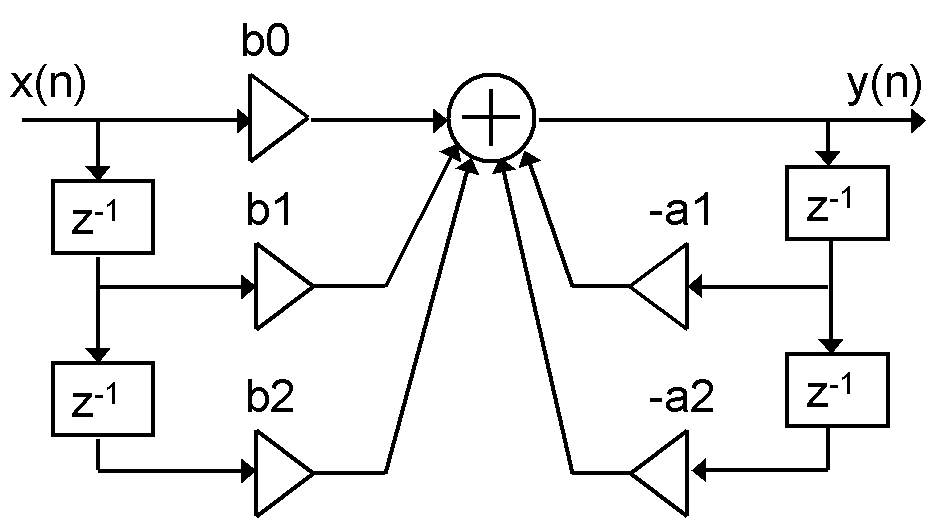
\includegraphics[width=0.5\textwidth]{biquadform1}
\caption{Biquad Direct Form 1.}
\label{fig:biquadform1}
\end{figure}

In Direct Form 1, you can reverse the position of the feedforward and -back delays by first splitting the summations. Then their order is switched, so that the feedback delays come first and the feedforward delays come second. This creates two pairs of the delays \(x(n-1)\) and \(x(n-2\) that are right after each other in operation. Therefore, one of the pairs are redundant, as the two pairs store the same information. Because of this, one of the pairs are removed \cite{Redmon2003}. This whole process can be seen in Figure \ref{fig:biquadtransform}. The new biquad structure is called Direct Form 2. The equation for this form is\cite{Nederland2016}:
\[y(n) = b_0 \cdot w(n) + b_1 \cdot w(n-1) + b_2 \cdot w(n-2)\]
\[w(n) = x(n) - a_1 \cdot w(n-1) - a_2 \cdot w(n_2)\]

\begin{figure}
\centering
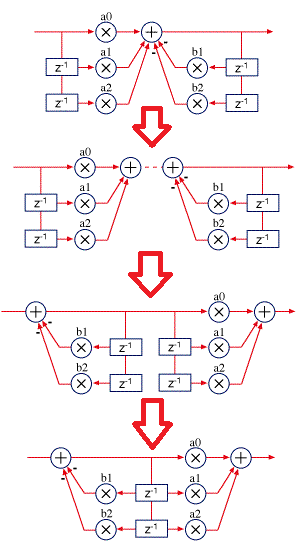
\includegraphics[width=0.5\textwidth]{directform2}
\caption{Biquad transformation from Direct Form 1 to Direct Form 2 \cite{Redmon2003}.}
\label{fig:biquadtransform}
\end{figure}

Direct Form 2 is better when working with floating points \cite{Redmon2003}. This is because it only saves two memory locations for the delays \(x(n-1)\) and \(x(n-2)\), which is more efficient than Direct Form 1 that saves four memory locations for its delays. Pure Data uses the Direct Form 2 structure. However, Pure Data defines the biquad differently, using the equation:
\[y(n) = b_0 \cdot w(n) + b_1 \cdot w(n-1) + b_2 \cdot w(n-2)\]
\[w(n) = x(n) + a_1 \cdot w(n-1) + a_2 \cdot w(n_2)\]

Because of this, the coefficients \(a_1\) and \(a_2\) are actually inversed, compared to the normal definition.

The bandpass filter works by letting certain frequencies pass through, while rejecting all other frequencies. The accepted frequencies are defined by having a band with width \(B\) and a frequency \(f_0\) as its  centre point. This structure can be seen in Figure \ref{fig:bandpass}. The outermost points of the band \(f_L\) and \(f_H\) define the lowest and highest frequencies that are passed through, respectively. All frequencies lower than \(f_L\) and higher than \(f_H\) are rejected \cite{zolzer2011dafx}.

\begin{figure}
\centering
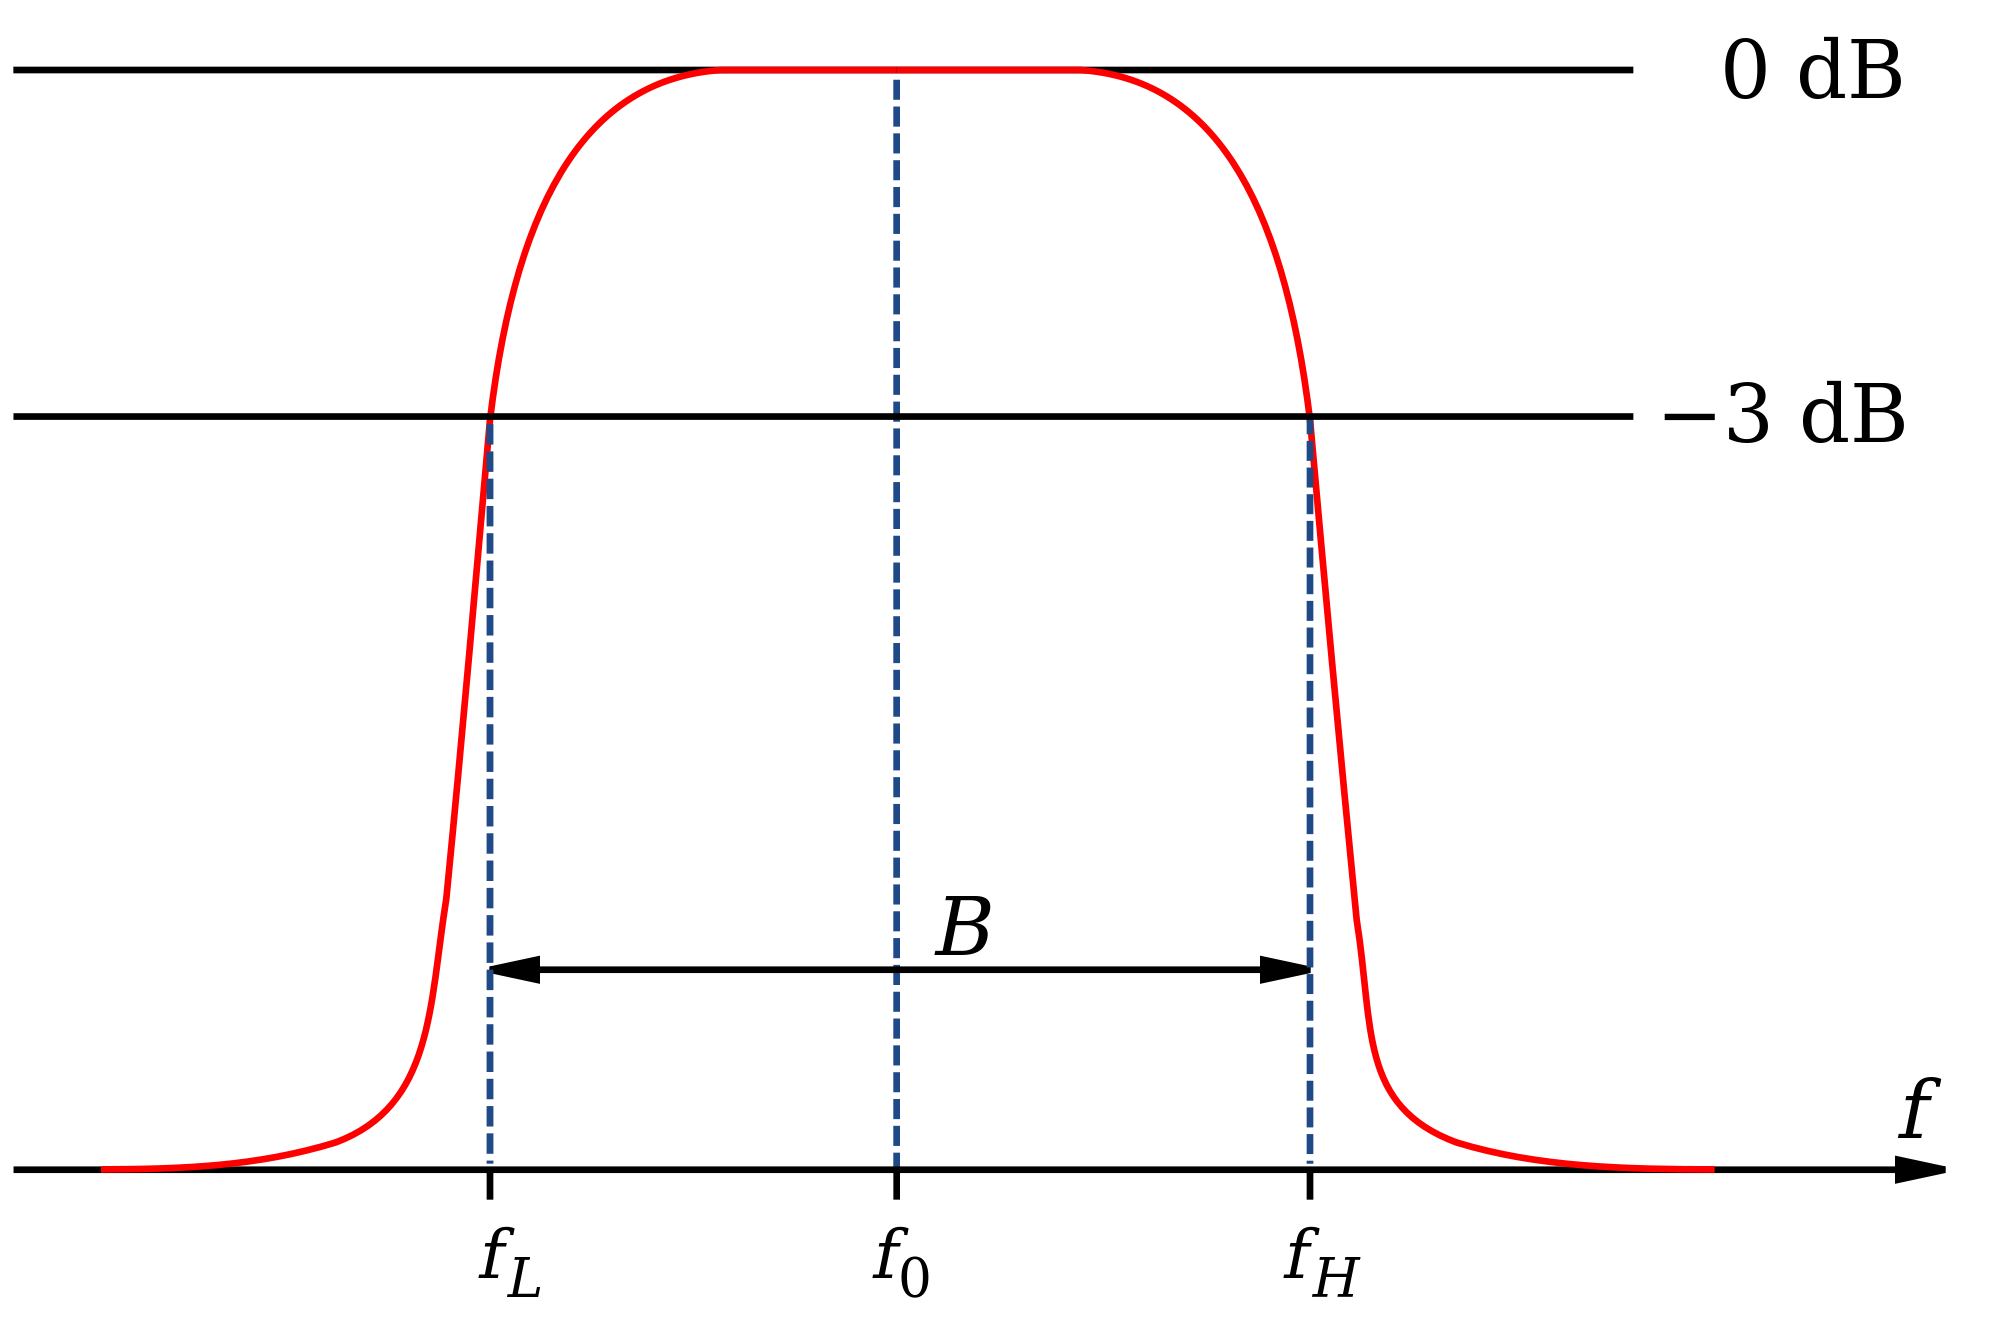
\includegraphics[width=0.5\textwidth]{bandpass}
\caption{Frequency response curve of a bandpass filter.}
\label{fig:bandpass}
\end{figure}

The high-shelf filter works by changing the amplitude of all frequencies that is higher than a defined threshold frequency. The amplitude change can be positive or negative, depending on the decibel gain defined by the filter coefficients\cite{zolzer2011dafx}. An example of the frequency response of a high-shelf filter can be seen in Figure .

\begin{figure}
\centering
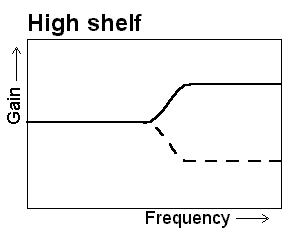
\includegraphics[width=0.5\textwidth]{highshelf}
\caption{Frequency response curve of a high-shelf filter.}
\label{fig:highshelf}
\end{figure}

\section{Software tools}\label{sec:softwareTools}
	\subsection{Image processing}\label{sub:imageprocessing}
	As the project revolves around pictures being audiolised, various image processing methods have been implemented. To get an image loaded into Pure data the library gem have been imported and applied. In gem it is possible to go through each pixel getting its RGB value as three different values. This is done using a double nested for-loop that is constructed using the expr function in Pure data, which allows for construction of consecutive if-statements. The first if-statement gives an output that is increased by 0.001 for every cycle if the input value is less than one. The second if-statement checks if the input value is greater or equal to one, if that is the case it adds 0.01 to a value starting at zero, which is then outputted. The last if-statement checks if the second input is greater or equal to 1, if that is the case subtract 1 from the value of the second input.
	
	Pipe is an object that delay the input given to it by a specific amount of milliseconds. It is used here to make sure that the program does not give a stack overflow error, and that it doesn't process the pixels too fast. By default in the program the pipe is set to 50 milliseconds since this allows the program to smoothly go through each pixel one by one. 
	When the pixel data is being processed in the program, it outputs the value of the three colour channels in the specific pixel, meaning that the output consists of three different value representing the R, G and B value. With the three RGB values it is possible to plot the values giving a graph of how the colour distribution is in the picture, but it is also possible to normalize the values into a signal by normalizing them from zero to one into negative one to positive one. By doing this the values have now been turned into a signal, which in terms should be able to produce a sound.

	\subsection{Audiolisation of image}\label{sub:audiolisationofimage} 
	Audiolisation of an image means to turn the image into some kind of audio, which is what the program explained in \ref{sub:imageprocessing} is programmed to do. 
	
	\subsection{Arduino}\label{sub:arduino}
	Arduino is a micro controller with open source software, that allows for custom coding in processing. Arduino has the capability to be connected to a breadboard for greater utility as the breadboard allows multiple components to be connected to a single Ardunio port, making it possible to create a 5 volt circuit using only a single pin. It is also possible to create a circuit using more than one pin, giving access to greater utility as each pin can be programmed separately in the program, giving each of the pins a unique functionality or making them become a duplicate, this would allow each pin to run a different circuit.
	Arduino is used in the project as the main control unit, as it is connects the physical interface to pure data. 
	
\section{Physical interface}\label{sec:physicalinterface}

	
	\subsection{Circuit diagram}\label{sub:circuitdiagram}
\begin{figure}
\centering
\includegraphics[width=0.5\textwidth]{circuit}
\caption{The circuit diagram.}
\label{fig:circuit}
\end{figure}

\begin{figure}
\centering
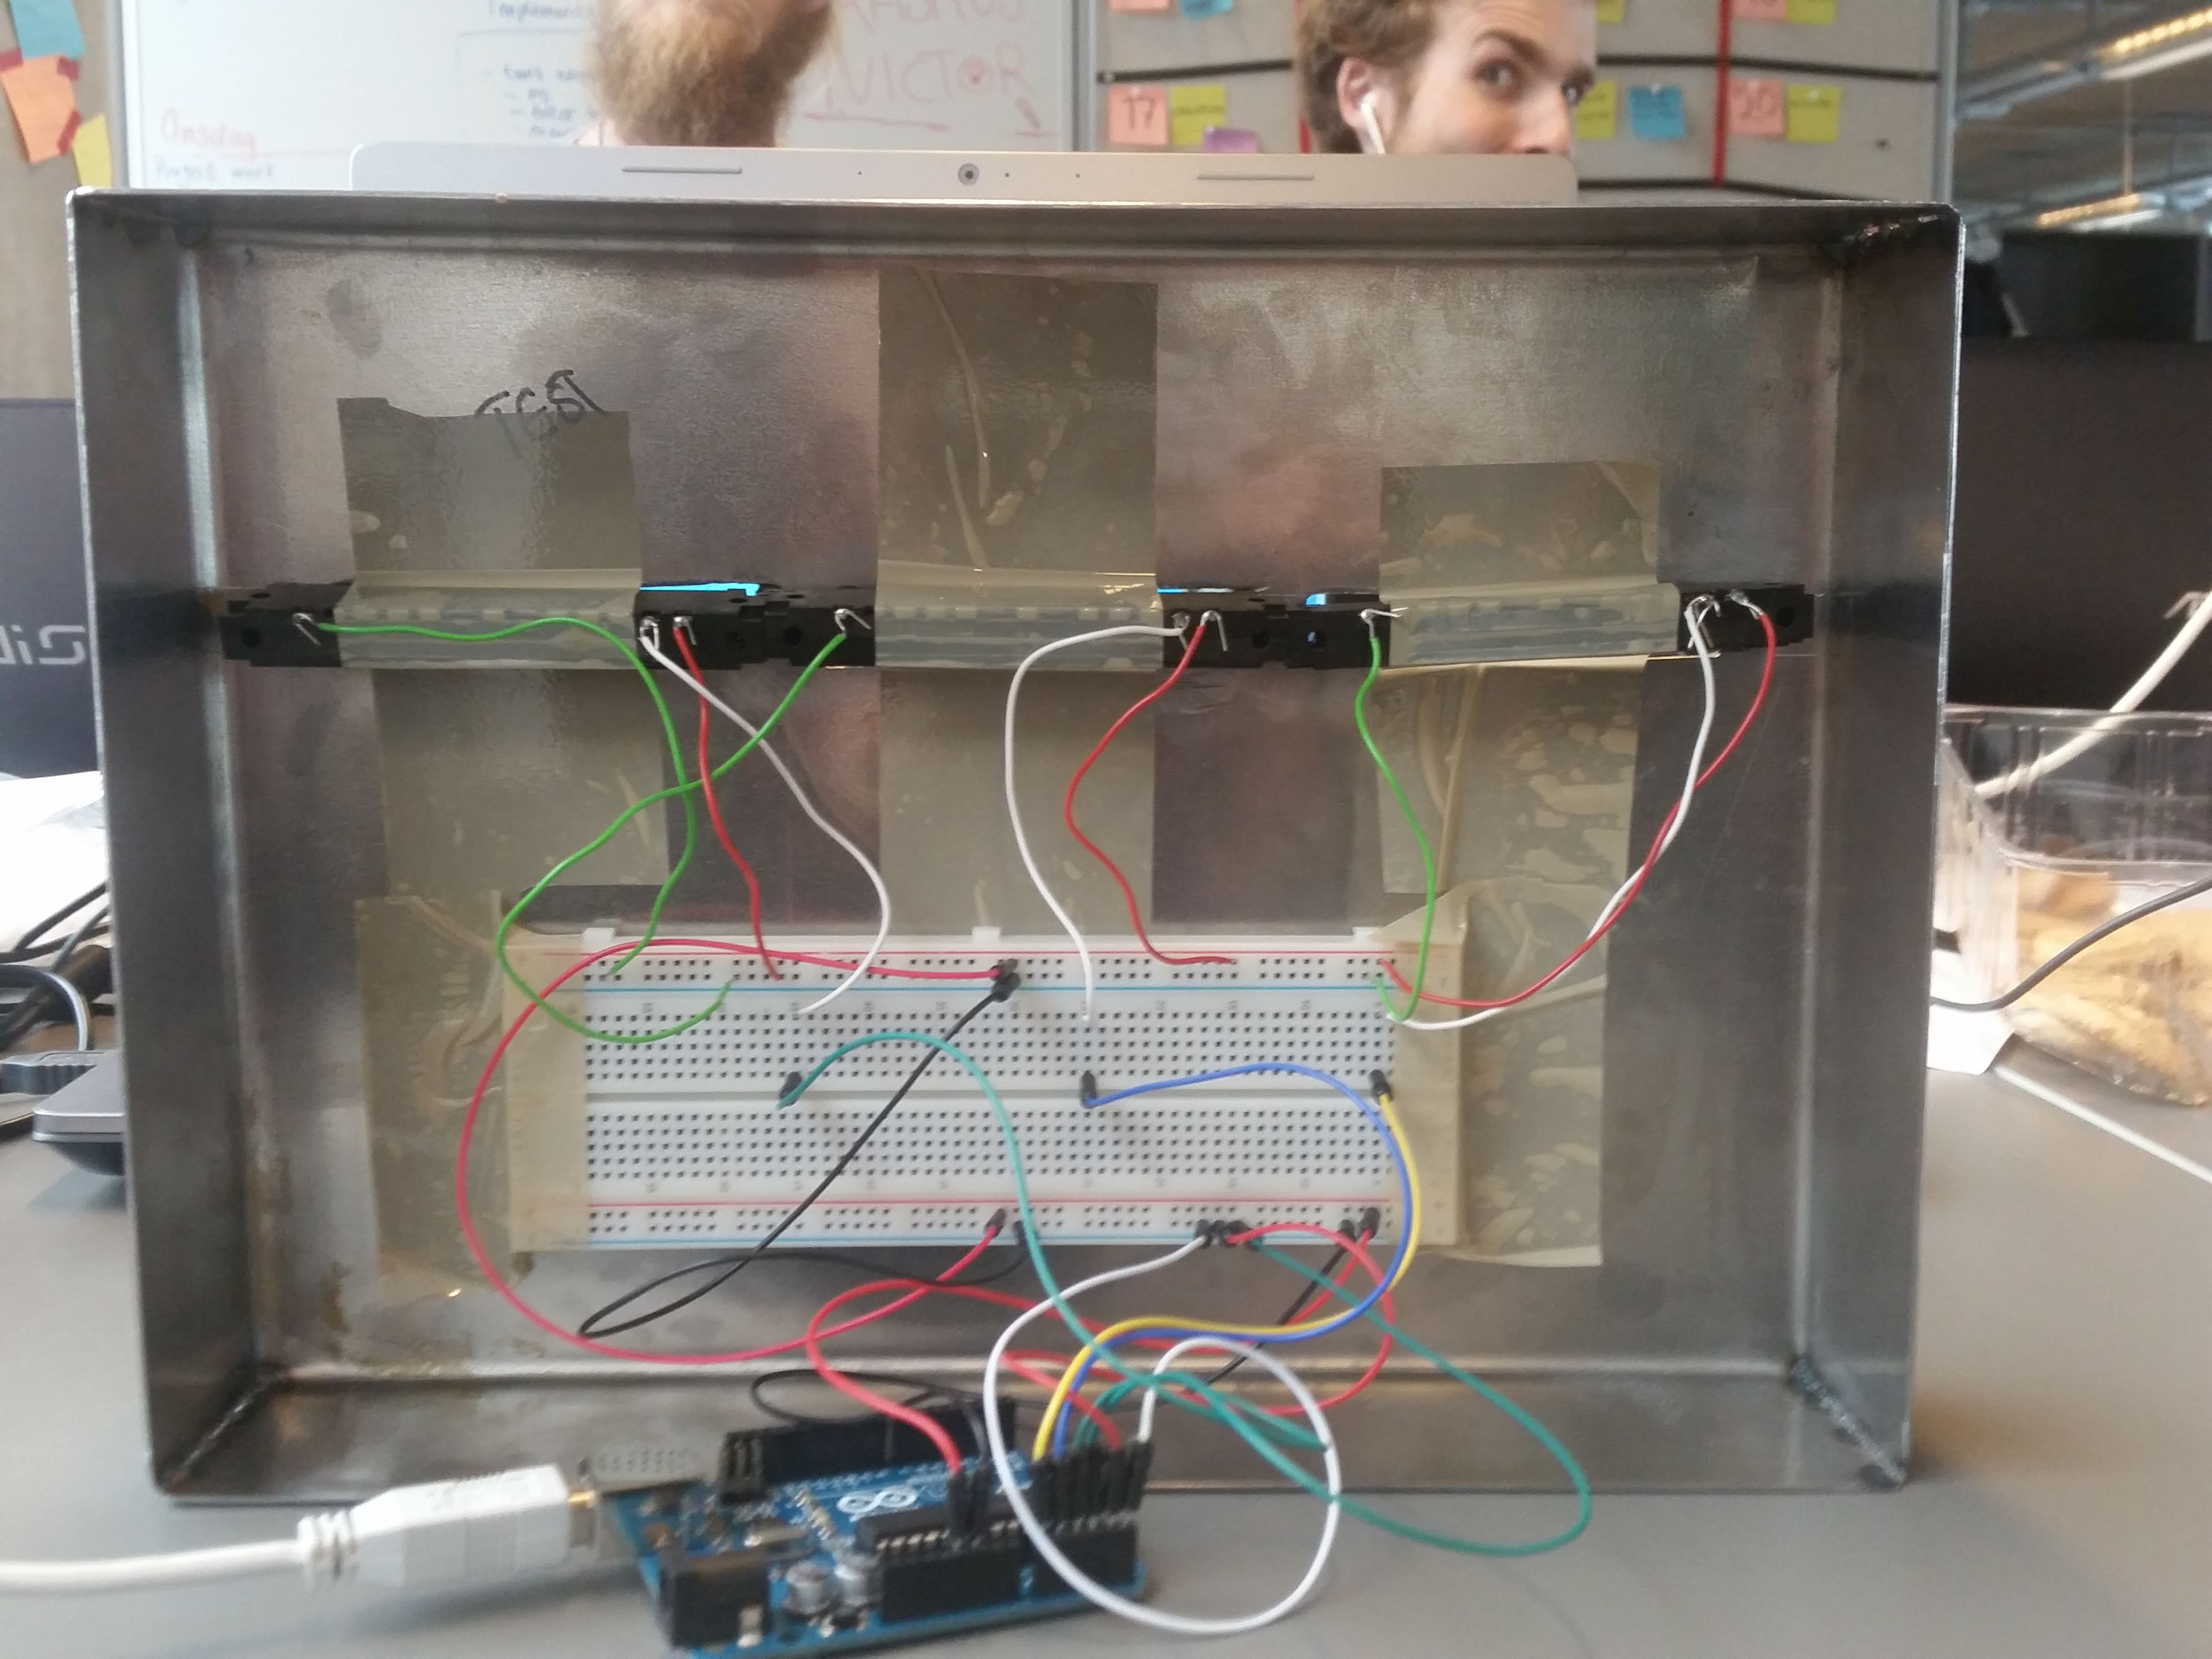
\includegraphics[width=0.5\textwidth]{backsideBox}
\caption{The circuit inside the box.}
\label{fig:backsideBox}
\end{figure}

\begin{figure}
\centering
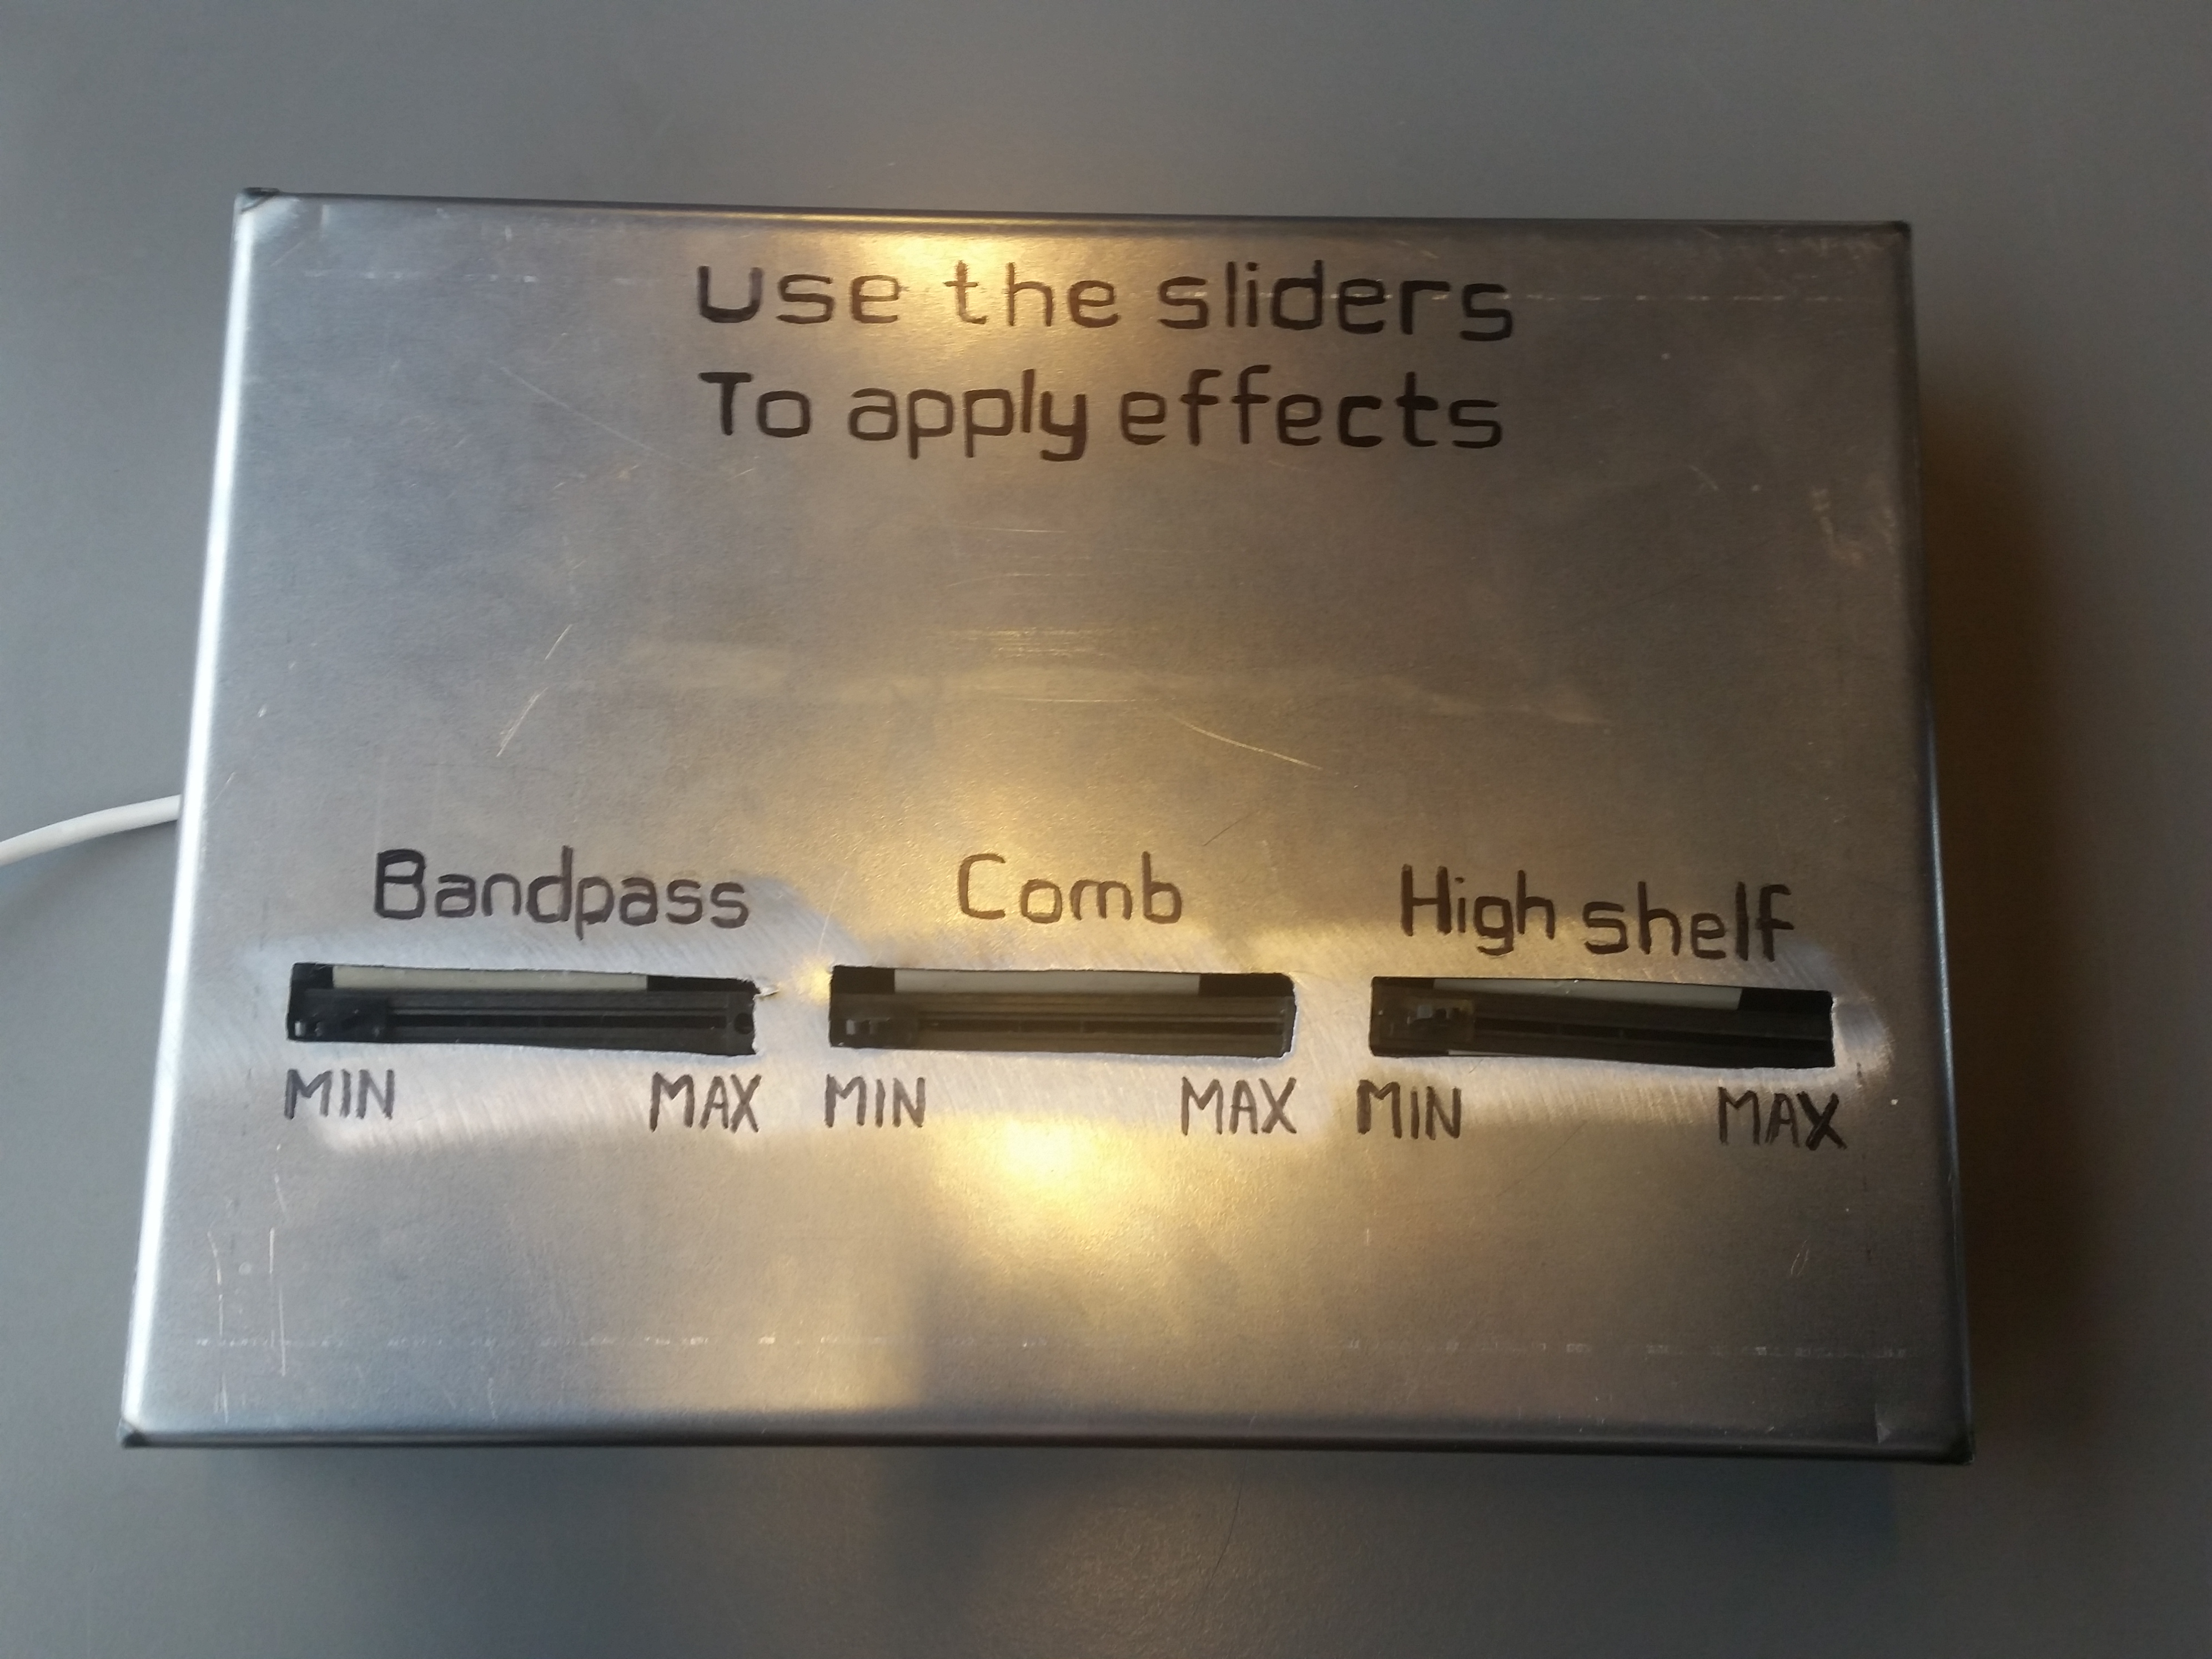
\includegraphics[width=0.5\textwidth]{frontBox}
\caption{The box containing the electronics.}
\label{fig:frontBox}
\end{figure}

	
	The interface utilises the Arduino's 5 volt power supply and three slide potentiometer that are placed in the lower half of the box. The slide potentiometers send their output to the Arduino's analogue ports, which is then interpreted by the code. This is elaborated upon in Chapter \ref{ch:codeoverview}.
